\documentclass[journal,12pt,twocolumn]{IEEEtran}
\usepackage[none]{hyphenat}
\usepackage{graphicx}
\usepackage{listings}
\usepackage[english]{babel}
\usepackage{graphicx}
\usepackage{caption} 
\usepackage{amsmath}
\usepackage{hyperref}
\usepackage{amsmath,amsfonts,amssymb}
\usepackage{booktabs}
\usepackage{array}
\let\vec\mathbf

\title{\textbf{\\Conics Assignment}}
\author{Sinkona Chinthamalla - FWC22054}

\newcommand{\myvec}[1]{\ensuremath{\begin{pmatrix}#1\end{pmatrix}}}
\newcommand{\mydet}[1]{\ensuremath{\begin{vmatrix}#1\end{vmatrix}}}
\providecommand{\brak}[1]{\ensuremath{\left(#1\right)}}
\providecommand{\lbrak}[1]{\ensuremath{\left(#1\right.}}
\providecommand{\rbrak}[1]{\ensuremath{\left.#1\right)}}
\providecommand{\sbrak}[1]{\ensuremath{{}\left[#1\right]}}

\begin{document}
\maketitle

\section{Question}
\textbf {Find the area of the region bounded by the curves $y=x^2+2$, $y=x$, $x=0$ and $x=3. $}

\begin{figure}[h!]
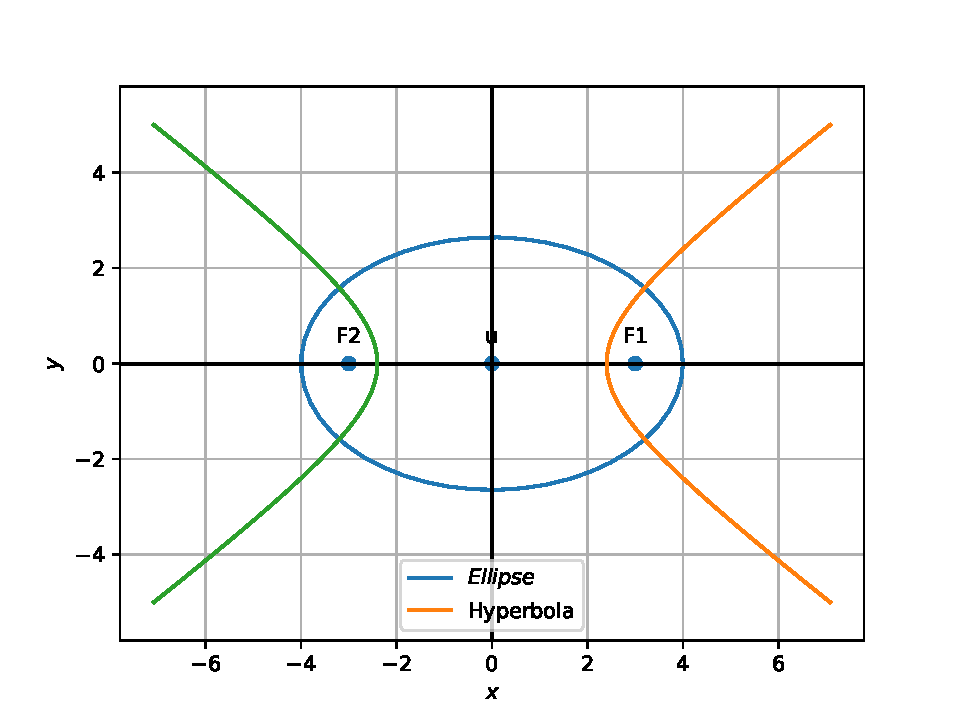
\includegraphics[scale=0.55]{conic1.pdf }
\end{figure}

\section{Construction}
\centering
\vspace{0.2cm}
{
\setlength\extrarowheight{2pt}
\begin{tabular}{|c|c|c|}
	\hline
	\textbf{Symbol}&\textbf{Value}&\textbf{Description}\\
	\hline
	\textbf{A} & 
	$ \begin{pmatrix}
      0 \\
      2
    \end{pmatrix}$ & $\vec{q_1} $\\
	\hline
	B & 
	$\begin{pmatrix}
     3 \\
     11
    \end{pmatrix}$ & $\vec{q_2} $\\
	\hline
	C & 
	$\begin{pmatrix}
     3 \\
     3
    \end{pmatrix}$ & $\vec{q_3} $\\
	\hline
	O & 
	$\begin{pmatrix}
     0 \\
     0
    \end{pmatrix}$ & $\vec{q_4} $\\
	\hline
\end{tabular}
}

\section{Solution}
\raggedright The equation of a conic with directrix $\vec{n}^\intercal\vec{x} = c$, eccentricity e and focus \textbf{F} is given by
\begin{align}
\vec{x}^{\top}\vec{V}\vec{x}+2\vec{u}^{\top}\vec{x}+f = 0 
\end{align}
where
\begin{align}
\vec{V} = \begin{pmatrix}
1 & 0\\
0 & 0
\end{pmatrix} \\
\vec{u} = \begin{pmatrix}
      0 \\
     -1/2
    \end{pmatrix}  \\
f = 2  
\end{align}

\textbf{Finding Points of Intersection}
\vspace{0.2cm}
\\1. Consider line 
\begin{align}
\begin{pmatrix}
 1 & 0
\end{pmatrix} \vec{x} = 0 \\ 
\vec{q_1} = y_1\vec{e_2} 
\end{align}

To find the point of intersection of the Parabola with (5), substitute (6) in (1)
\begin{align}
\vec{q_1}^{\top}\vec{V}\vec{q_1}+2\vec{u}^{\top}\vec{q_1}+f = 0 \\
y_1^2\vec{e_2}^{\top}\vec{V}\vec{e_2}+2y_1\vec{u}^{\top}\vec{e_2}+f = 0 
\end{align}  
The value of $y_1$ is given by \\
\vspace{0.2cm}
1. when $\vec{e_2}^{\top}\vec{V}\vec{e_2} \neq 0 $ 
\begin{align}
y_1=\frac{-b_1 \pm \sqrt{b_1^2-4a_1c_1}}{2a_1} 
\end{align}
where,
\begin{align*}
a_1 & = \vec{e_2}^{\top}\vec{V}\vec{e_2}  \\
b_1 & = 2\vec{u}^{\top}\vec{e_2}  \\
c_1 & = f
\end{align*}

\vspace{0.2cm}
2. when $\vec{e_2}^{\top}\vec{V}\vec{e_2} = 0 $ 
\begin{align}
y_1=\frac{-f}{2\vec{u}^{\top}\vec{e_2}} 
\end{align} 

From (2) and $\vec{e_2}$, $\vec{e_2}^{\top}\vec{V}\vec{e_2} = 0 $ \\
Therefore, $y_1$ is obtained by substituting (3), (4) and $\vec{e_2}$ in (10).

\vspace{0.4cm}
2. Now consider line 
\begin{align}
\begin{pmatrix}
 1 & 0
\end{pmatrix} \vec{x} = 3 \\
\vec{q_2} = y_2\vec{e_2}+3\vec{e_1}
\end{align}

To find the point of intersection of the Parabola with (11), substitute (12) in (1)
\begin{align}
\vec{q_2}^{\top}\vec{V}\vec{q_2}+2\vec{u}^{\top}\vec{q_2}+f = 0 
\end{align}
\begin{equation*}
y_2^2\vec{e_2}^{\top}\vec{V}\vec{e_2}+3y_2\vec{e_2}^{\top}\vec{V}\vec{e_1}+3y_2\vec{e_1}^{\top}\vec{V}\vec{e_2}+9\vec{e_1}^{\top}\vec{V}\vec{e_1}
\end{equation*}
\begin{equation}
+2y_2\vec{u}^{\top}\vec{e_2}+6\vec{u}^{\top}\vec{e_1}+f = 0 
\end{equation}

\vspace{0.2cm}
The value of $y_2$ is given by \\
\vspace{0.2cm}
1. when $\vec{e_2}^{\top}\vec{V}\vec{e_2} \neq 0 $ 
\begin{align}
y_2=\frac{-b_2 \pm \sqrt{b_2^2-4a_2c_2}}{2a_2} 
\end{align}
where,
\begin{align*}
a_2 & = \vec{e_2}^{\top}\vec{V}\vec{e_2}\\
b_2 & = 3\vec{e_2}^{\top}\vec{V}\vec{e_1}+3\vec{e_1}^{\top}\vec{V}\vec{e_2}+2\vec{u}^{\top}\vec{e_2} \\
c_2 & = 9\vec{e_1}^{\top}\vec{V}\vec{e_1}+6\vec{u}^{\top}\vec{e_1}+2 
\end{align*}

\vspace{0.2cm}
2. when $\vec{e_2}^{\top}\vec{V}\vec{e_2} = 0 $ 
\begin{align}
y_2=\frac{-f-9\vec{e_1}^{\top}\vec{V}\vec{e_1}}{2\vec{u}^{\top}\vec{e_2}} 
\end{align} 

From (2) and $\vec{e_2}$, $\vec{e_2}^{\top}\vec{V}\vec{e_2} = 0 $\\
Therefore, $d_2$ is obtained by substituting (2), (3), (4), $\vec{e_1}$ and $\vec{e_2}$ in (16). 

\vspace{0.4cm}
Therefore, the Points of Intersection of (5) and (11) with the given parabola are
\begin{align}
\vec{q_1} = \begin{pmatrix}
 0\\
 2
\end{pmatrix} 
\end{align}
and 
\begin{align}
\vec{q_2} = \begin{pmatrix}
 3\\
 11
\end{pmatrix} 
\end{align}
respectively.

\vspace{0.2cm}
The Points of Intersection of (11) and (5) with the line
\begin{align}
\begin{pmatrix}
 1 & -1
\end{pmatrix} \vec{x} = 0
\end{align}  are
\begin{align}
\vec{q_3} = \begin{pmatrix}
 3\\
 3
\end{pmatrix} 
\end{align}
\begin{align}
\vec{q_4} = \begin{pmatrix}
 0\\
 0
\end{pmatrix} 
\end{align}
and

respectively.

\vspace{0.2cm}
\textbf{Finding area of the bounded region} \\
From Fig. 1, the area covered by the parabola is given by
\begin{align}
\int_{0}^{3} (x^2+2)dx =  \frac{x^3}{3} + 2x \Big|_0^3 \\
=15 
\end{align}

The area covered by (19) is given by
\begin{align}
\int_{0}^{3} xdx =  \frac{x^2}{2} \Big|_0^3 \\
= \frac{9}{2}
\end{align}

Thus, the desired area is the bounded region in
\\Fig. 1, and is given by
\begin{align}
\frac{21}{2} \quad sq.units
\end{align}

%\vspace{0.2cm}
%Get the python code from
%\begin{table}[h]
%\large
%\centering
%\begin{tabular}{|l|}
%\hline
%https://github.com/SinkonaChinthamalla/fwc/
%\\blob/main/matrix/conics/codes \\
%\hline
%\end{tabular}
%\end{table}	
\end{document}